\ProvidesFile{chapters/ch-Cross_Section_Measurement.tex}

\chapter{MEASUREMENTS OF DIFFERENTIAL CROSS-SECTIONS}
\label{Measurements_of_Differential_Cross-sections}
The measurements follow the analysis strategy of CMS TOP-18-006~\cite{Sirunyan:2681777}, but has been extended with additional observables, differential measurements as a function of \ttbar invariant mass, several optimizations that reduce systematic uncertainties, and significantly increased luminosity.
All measured distributions are corrected for detector efficiencies and acceptances and extrapolated to parton-level using a regularized unfolding procedure with detector response obtained from MC simulated SM predictions with NLO matrix element accuracy with parton-shower algorithms.
The spin density coefficients are extracted from the unfolded distributions, constituting a precision test of the SM.

\section{Reconstructed Top Quark Polarization and \ensuremath{\mathrm{t\bar{t}}} Spin Correlation Observables}
\label{Reconstructed_Polarization_Spin_Correlation_Observables}
Top quark polarization and \ttbar spin correlation observables $\cos\theta_{1(2)}^i$, $\cos \theta_1^i \cos \theta_2^i$, and $\cos \theta_1^i \cos \theta_2^j \pm \cos \theta_1^j \cos \theta_2^i$ are calculated using reconstructed top quarks and leptons as described in section~\ref{Top_Quark_Polarizations_and_ttbar_Spin_Correlations}, where the quantity $\cos \theta_1^k = \hat{\bar{\ell}}_1 \cdot \hat{k}$, as an example, can be calculated by taking the dot product of the charged anti-lepton direction in its grandfather top quark's ZMF with the $\hat{k}$ helicity basis spin quantization axis in the \ttbar ZMF.
Additionally, the following distributions are also measured:
\begin{itemize}
    \item Top quark polarization and \ttbar spin correlation observables with modified axes $\hat{r^*}$ and $\hat{k^*}$, equal to $\pm \hat{r}$ or $\pm \hat{k}$ depending on $\operatorname{sign}(\vert y_t \vert-\vert y_{\bar{t}} \vert)$, due to their sensitivity to SMEFT dimension-six operators
    \item Linear Combinations of spin correlation observables $-\cos \theta_1^i \cos \theta_2^i \mp \cos \theta_1^j \cos \theta_2^j - \cos \theta_1^l \cos \theta_2^l$ and $-\cos \theta_1^i \cos \theta_2^j \mp \cos \theta_1^j \cos \theta_2^i - \cos \theta_1^l \cos \theta_2^l$ that have linear single-differential cross-sections in the full phase space with coefficients $-C_{ii} \mp C_{jj} - C_{ll}$ and $-C_{ij} \mp C_{ji} - C_{ll}$
    \item  $\cos\varphi=\hat{\bar{\ell}}_{1} \cdot \hat{\ell}_2$, the dot product of the charged lepton directions in their grandfather top quark's ZMF, sensitive to coefficient $D = -\frac{1}{3}Tr[\matr{C}] = -\frac{1}{3}(C_{kk} + C_{rr} + C_{nn})$ with single-differential cross-section $\tfrac{1}{\sigma}\tfrac{d\sigma}{d\cos\varphi} = \tfrac{1}{2}(1-D\cos\varphi)$
    \item $\cos\varphi_{\mathrm{lab}}=\hat{\bar{\ell}}^{lab}_1 \cdot \hat{\ell}^{lab}_2$, as above but using lepton directions measured in the laboratory frame
    \item Lab frame observables $\vert \Delta\phi_{\ell\bar{\ell}} \vert$ ($\vert \Delta\eta_{\ell\bar{\ell}} \vert$), the difference in azimuthal angle $\phi$ (pseudorapidity $\eta$) between the two leptons in the lab frame, which are indirectly sensitive to the spin density coefficients and have excellent experimental resolution
\end{itemize}
Moreover, all measured distributions are measured both in the full selected phase space and differentially, with the phase space partitioned in bins of \ttbar invariant mass $m_{\ttbar}$.
The differential measurements are well-motivated based on the revelations discussed in section~\ref{Top_Quark_Spin_in_ttbar_Production_and_Top_Decay}, that the kinematic and spin properties of a \ttbar pair can be completely described at LO in the \ttbar ZMF by the invariant mass $m_{\ttbar}$ and the top scattering angle $\Theta$.

\section{Background Subtraction}
\label{Background_Subtraction}
Prior to unfolding, the predicted MC simulated signal and background rates are used to subtract the estimated background contributions in each bin of distributions measured with recorded data:
\begin{linenomath*}
\begin{align}
N^{Signal}_{Data} = N^{Total}_{Data} \times \frac{N^{Signal}_{MC}}{N^{Total}_{MC}}.
\label{Data_Background_Subtraction}
\end{align}
\end{linenomath*}
Subtracting the estimated background from the measured data prior to unfolding reduces the impact of the unwanted backgrounds contributions and improves the accuracy of the unfolding procedure.
Uncertainties on the subtracted background contributions are propagated to the remaining signal contributions.

\section{Acceptance, Efficiency, Smearing, Purity, and Stability}
The CMS detector has limited acceptance and reconstruction efficiency as well as finite resolution.
Acceptance refers to the total number of events or particles that can be detected within the geometric coverage of the detector, and efficiency is the fraction of those events or particles that are reconstructed.
The acceptance$\times$efficiency is described by diagonal matrix $\matr{A}$, in each bin of the true distribution, with 
The smearing of events between bin is described by matrix $\matr{S}$, due to finite detector resolution and imperfect reconstruction techniques.
The $\matr{A}$ and $\matr{S}$ matrices can be quantified as:
\begin{linenomath*}
\begin{align}
\matr{A}_{ij} = \frac{N_{ \{ x_i \} \cap \{ \vec{y} \}}}{N_{ \{ x_i \} }} \quad \quad
\matr{S}_{ij} = \frac{N_{ \{ y_j \} }}{N_{ \{ x_i \} \cap \{ \vec{y} \}}}
\end{align}
\end{linenomath*}
where $N_{ \{ x_i \} \cap \{ \vec{y} \}}$ is the number of events generated in the $i$th bin that were reconstructed in any bin, $N_{ \{ x_i \} }$ is the number of events generated the $i$th bin, and $N_{ \{ y_j \} }$ is the number of events reconstructed in the $j$th bin.

The migration of events between bins due to smearing is also characterized by measures of purity of stability.
Purity refers to the fraction of events in the reconstructed detector-level distribution that were actually generated in the same bin of the true generator-level distribution, with a high (low) purity for a bin indicating that a small (large) number of events in that bin of the reconstructed detector-level distribution migrated in from other bins in the true generator-level distribution.
Stability refers to the fraction of events in a bin of the true generator-level distribution that were reconstructed in the same bin, with a high (low) stability indicating that a small (large) number of events in that bin of the true generator-level distribution migrated out to other bins of the of the reconstructed detector-level distribution.
Purity and stability can be quantified as:
\begin{linenomath*}
\begin{align}
(\text{Purity})_i = \frac{N_{ \{ x_i \} \cap \{ y_i \} }}{N_{ \{ y_i \} }} \quad \quad
(\text{Stability})_i = \frac{N_{ \{ x_i \} \cap \{ y_i \} }}{N_{ \{ x_i \} \cap \{ \vec{y} \}}}
\end{align}
\end{linenomath*}
where $N_{ \{ y_i \} }$ is the number of events reconstructed in the $i$th bin, $N_{ \{ x_i \} \cap \{ \vec{y} \}}$ is the number of events generated in the $i$th bin that were reconstructed in any bin, and $N_{ \{ x_i \} \cap \{ y_i \} }$ is the number of events generated in the $i$th bin that were also reconstructed in the $i$th bin.

\section{Unfolding Procedure}
The event selection criteria and analysis techniques such as the \ttbar kinematic reconstruction trade acceptance and efficiency in exchange for a high purity of signal events.
As a result, measured bins of reconstructed detector-level distributions $\vec{y}$ are distorted from the true generator-level distributions $\vec{x}$ by acceptance, efficiency, and bin-to-bin migrations:
\begin{linenomath*}
\begin{align}
\vec{y}_{\text{MC}} = \matr{M} \vec{x}_{\text{MC}} \quad \quad \xrightarrow[\text{Unfolding}]{\text{Naive}} \quad \quad \vec{x} = \matr{M}^{-1} \vec{y}
\end{align}
\end{linenomath*}
where $\matr{M}$ is the response-matrix constructed from $\matr{A}$ and $\matr{S}$.
To correct the bin of background-subtracted recorded data distributions for smearing and acceptance effects, the TUnfold~\cite{TUnfold} package of the ROOT data analysis framework is used to simultaneously invert $\matr{M}$ and unfold the detector-level distributions $\vec{y}$ of recorded data into distributions $\vec{x}$ that have been corrected for bin migrations and extrapolated to parton-level.
The response-matrices $\matr{M}$ are constructed using signal process events from the $\Powheg + \Pythia$ MC simulation including smearing from the \Geant-simulated detector response.
For each measured observable, the response-matrices are two-dimensional, reconstructed detector-level versus true generator-level distributions containing events that pass the event selection.
In each generator-level bin, the true generated events in that bin that do not pass the event selection are filled in the underflow.
For each measured distribution, the absolute differential cross-section, the differential cross-section normalized to unit area, and the extracted spin-density coefficients constitute the final results of the unfolding procedure.

\subsection{Regularization}
\label{Regularization}
Regularized unfolding is used to suppress statistical fluctuations and reduce the impact of noise by introducing a term into the unfolding algorithm that incorporates assumptions that constrain the unfolded result to be smoother.
This technique helps prevent over-fitting data and improves the stability of the unfolded result.
The unfolding for these measurements is performed using the TUnfoldDensity class~\cite{TUnfold}, which offers greater control over the regularization, using a $\chi^{2}$ fit to simultaneously invert $\matr{M}$ and regularize the unfolded result:
\begin{linenomath*}
\begin{align}
\chi^{2}_{unf}&=\chi^{2}_{\matr{M}}+\tau^{2}\chi^{2}_{\matr{L}}+\lambda\sum_{i}(\matr{M}\vec{x}-\vec{y})_{i} \\
\mathrm{where \quad} \chi^{2}_{\matr{M}}&=(\matr{M}\vec{x}-\vec{y})^{T}\matr{V}_{y}^{-1}(\matr{M}\vec{x}-\vec{y}) \\
\chi^{2}_{\matr{L}}&={(\vec{z})}^{T}\matr{L}^{T}\matr{L}{(\vec{z})} \quad \text{where} \quad z_i = f_i \cdot (x_i - c \cdot x^{\text{MC}}_i)
\label{eq:Chi2TUnfold}
\end{align}
\end{linenomath*}
where $\matr{V}_{y}$ is the diagonal covariance matrix of the reconstructed detector-level distribution $\vec{y}$, $\matr{L}$ is a matrix specifying the regularization conditions, and .

The $\chi^{2}_{\matr{M}}$ term is a least squares fit of the re-folded output $\matr{M}\vec{x}$ to the original data $\vec{y}$.
In the absence of the other terms, the unfolded result will often have unacceptably large statistical fluctuations arising from strong anti-correlations between adjacent bins, and thus the expected shape $\vec{x}_{\text{MC}}$ of the distribution is used to regularize the output via the $\chi^{2}_{\matr{L}}$ term, with the strength of the regularization controlled by the $\tau$ parameter. 
Larger (smaller) values of $\tau$ mean the unfolded output will be over-smoothed (noisy) and more (less) strongly constrained by the generator-level MC vector $\vec{x}_{\text{MC}}$).
For each unfolded result, the value of $\tau$ is chosen by scanning for the $\tau$ that yields the minimum of $\rho_{avg}$, the mean of the global correlation coefficient $\rho_{i}$ in the bins of the unfolded distribution:
\begin{linenomath*}
\begin{align}
\rho_{i} = \sqrt{1 - \frac{1}{[{(\matr{V}_{x}))}_{ii} \cdot {(\matr{V}_{x})^{-1})}_{ii}]}} \quad \text{with} \quad 0 \leq \rho_{i} \leq 1
\end{align}
\end{linenomath*}
where $\matr{V}_{x}$ is the covariance matrix of the unfolded result $\vec{x}$ obtained through standard propagation of errors in the linear transformation of the reconstructed distribution $\vec{y}$ into $\vec{x}$, specified in equation~\ref{eq:Chi2TUnfold}.
The $\lambda\Sigma_{i}(\matr{M}\vec{x}-\vec{y})_{i}$ term is a Lagrange multiplier that ensures the integral of the re-folded output matches that of the input.

For the unfolded measurements presented in this dissertation, the $\matr{L}$ matrix is chosen such that the regularization minimizes the curvature of the difference between the unfolded distribution $\vec{x}$ and the generator-level MC distribution $c*\vec{x}_{\text{MC}}$, where $c$ is a scale factor that normalizes the total number of reconstructed-level MC signal events to number observed in recorded data.
Curvature regularization is unbiased when the shape of $\vec{x}$ can only differ from the shape of the MC simulation $c*\vec{x}_{\text{MC}}$ by a linear function of the measured variable. 
This is true for observables such as $\cos\theta$, where the SM analytical form of the differential cross-section are known to depend linearly on the measured coefficient $B$: $\tfrac{1}{\sigma}\tfrac{d\sigma}{d\cos\theta} = \tfrac{1}{2} (1+B \cos\theta)$. 

In order for the curvature matrix $L$ to provide unbiased regularization for observables with differential cross-sections that have non-linear dependence, TUnfoldDensity allows for the inclusion of bin factor functions in the regularization term, with an appropriate $f_i$ calculated for each bin such that $f_i \cdot (x_i - c \cdot x^{\text{MC}}_i)$ depend linearly on the measured coefficient. 
The function $f(x)$ is calculated with $g(x) - g_{\text{MC}}(x)$, the continuous analogue of $(x_i - c \cdot x^{\text{MC}}_i)$, such that $z(x) = f(x) \cdot (g(x) - g_{\text{MC}}(x)) = \mathrm{constant} \times x$, where $g(x)$ is the functional form of the unfolded distribution and $g_{\text{MC}}(x)$ is the functional form of the generated-level distribution in MC simulation (which assumes the SM value of the specific spin-density coefficient).
The functional form of the distribution $g(x) = \tfrac{1}{\sigma}\tfrac{d\sigma}{dx}$ is known (see section ~\ref{Top_Quark_Polarizations_and_ttbar_Spin_Correlations}) for each of the observables measured in the top rest frame:
\begin{linenomath*}
\begin{align}
x=\cos\theta_1^i, \:\: g(x) &= \frac{1}{\sigma}\frac{d\sigma}{dx} = \frac{1}{2} (1+B_1^{i} x) \\ 
x=\cos\theta_1^i\cos\theta_2^i, \:\: g(x) &= \frac{1}{\sigma}\frac{d\sigma}{dx} = \frac{1}{2} (1-C_{ii} x) \log \left(\frac{1}{\left \vert x \right \vert }\right) \\ 
x=\cos\theta_1^i\cos\theta_2^j\pm \cos\theta_1^j\cos\theta_2^i, \:\: g(x) &= \frac{1}{\sigma}\frac{d\sigma}{dx} = \frac{1}{2} \left( 1 - \frac{C_{ij} \pm C_{ji}}{2} \, x \right)  \cos ^{-1}\left \vert x \right \vert \\
\end{align}
\end{linenomath*}
Then, $f(x) \propto \frac{x}{g(x)-g_{\text{MC}}(x)}$ follows:
\begin{linenomath*}
\begin{align}
x=\cos\theta_1^i, \:\: f(x) &= 1 \\
x=\cos\theta_1^i\cos\theta_2^i, \:\: f(x) &= \frac{1}{\log \left(\frac{1}{\left\vert x \right \vert }\right)} \\
x=\cos\theta_1^i\cos\theta_2^j\pm \cos\theta_1^j\cos\theta_2^i, \:\: f(x) &=  \frac{1}{\cos ^{-1}\left \vert x \right \vert}
\end{align}
\end{linenomath*}
All the distributions $g(x)$ considered are parameterized by only on a single coefficient, so $f(x)$ never has any dependence on any model parameters and the regularization is always unbiased, even if NP contributions are present in the recorded data. 
The choice of constant factor for $f(x)$ is inconsequential, as it is reabsorbed into the value of $\tau$, and is arbitrarily chosen such that the average value of the distribution is unity.
To apply the derived continuous bin factor functions to the binned distributions, $f(x)$ must integrated over the boundaries of each bin to calculate the appropriate $f_i$ for that bin. 

For the observables measured in the laboratory frame ($\cos\varphi_{\mathrm{lab}}$, $\vert \Delta\phi_{\ell\bar{\ell}} \vert$, and $\vert \Delta\eta_{\ell\bar{\ell}} \vert$), analytical forms of the differential cross-sections are not known. 
Furthermore, the distributions depend on more than a single coefficient, so the regularization cannot be made perfectly unbiased with respect to all of them simultaneously. 
Fortunately, because the migration matrix is almost diagonal, the chosen regularization strength for these variables is so weak that the choice of $f$ makes little difference. 
Analogous to the top rest frame observables, $f(x)$ is set equal to the reciprocal of the symmetrized SM distribution $1/\mathrm{SM_{sym}}(x)$, so that the regularization is unbiased to variations of the form $x \mathrm{SM_{sym}}(x)$. 

For differential unfolding of the observables as a function of $m_{\ttbar}$, TUnfold "unwraps" the two-dimensional distributions into one-dimensional distributions and the unfolding procedure is performed similarly to as previously described. 
TUnfold allows regularization along the axis of the observable to prevent spurious statistical fluctuations as discussed before, while not regularizing along the $m_{\ttbar}$ axis, as its functional form is not known.


\subsection{Binning}
\label{Binning}
Binning schemes for all distributions and matrices need to be chosen such that the resolution of the measured quantities are comparable to the bin widths.
A binning scheme of six uniform bins $[-1,-\frac{2}{3},-\frac{1}{3},0,+\frac{1}{3},+\frac{2}{3},+1]$ is shown to match the measurement resolution for all spin density coefficient distributions, and for differential measurements in $m_{\ttbar}$, four bins are used to partition the phase space $[250,450,600,800,\infty] \; \si{\GeV}$.
To avoid having zero degrees of freedom in the least-squares term of $\chi^{2}_{Unf}$, reconstructed detector-level distributions are required to have twice as many bins as the true generator-level distributions.

With any binning scheme, information about the dependence of acceptance, efficiency, and migration inside each bin is lost, so the unfolding will be inherently biased.
By unfolding with a finer binning scheme, more information is retained, the bias can be mitigated, and the precision improved.
The unbiased regularization method means finer bins can be used without concern that the explicit regularization of the curvature might cause more bias than the implicit regularization from binning.
To assess this, linearity tests are performed by injecting the distributions with changes in the spin-density coefficients by reweighting the simulated MC events and measuring the response of the unfolded results.
Finer binning by a factor of four ($24 = 6 \cdot 4$ bins) is found to have near-perfect linearity and remove most of the implicit bias for one-dimensional unfolding, while for two-dimensional unfolding finer binning by a factor of two ($12 \times 8 = 6 \cdot 2 \times 4 \cdot 2$ bins) along each axis is found to be a good trade-off between removing bias and over-binning.
To prevent the measurement sensitivity to features in the data smaller than the experimental resolution, the output distribution is re-binned immediately after the $\chi^2$ fit and $\tau$ scan is performed with the original binning.

\section{Conversion to Differential Cross-Sections}
The $i$th bin of the absolute differential cross-sections are obtained from the unfolded distributions $\vec{x}$ as:
\begin{linenomath*}
\begin{align}
(\frac{d\sigma}{dx})_i = \frac{1}{\Delta x_i} \frac{x_i}{BF \cdot \mathcal{L}} 
\end{align}
\end{linenomath*}
where $\Delta x_i$ is the bin width, $BF$ is the branching fraction of the \ttbar decay mode and channel, and $\mathcal{L}$ is the integrated luminosity.
Dividing by the total \ttbar production cross-section $BF \cdot \mathcal{L} \cdot \sum_i x_i$ normalizes the absolute differential cross-sections to unity:
\begin{linenomath*}
\begin{align}
(\frac{d\sigma}{dx})_i = \frac{1}{\Delta x_i} \frac{x_i}{\sum_i x_i} 
\end{align}
\end{linenomath*}
which is independent of $BF$ and $\mathcal{L}$, as these factors only effect the total rate of the distribution and not the shape.



\section{Systematic Uncertainties}
\label{Systematic_Uncertainties}
Each systematic uncertainty is evaluated in every measurement bin by repeating the full analysis with up and down $\pm \; 1 \sigma$ variations of an input parameter or event weight correction factor.
For each systematic source, the difference between the varied result and the nominal result provides the uncertainty.
For systematics that have many highly-correlated contributions, the combined impact of all contributions is obtained by enveloping largest difference between the nominal value and varied results in each bin.
The total up and down systematic uncertainties in each bin is then obtained by adding the uncorrelated systematic uncertainties in quadrature.
The averaged differences of the total up and down variations in each bin from the nominal provides the final estimate of the total systematic uncertainty.

\subsection{Experimental Systematics}
\label{Experimental_Systematics}
Experimental systematic uncertainties arise from detector imperfections and limitations of data analysis techniques.
Sources of experimental systematic uncertainties include detector response, object reconstruction, efficiencies, background modeling, calibrations, and alignment.
\begin{itemize}
    \item {\bf Luminosity} \\
    The measurement uncertinaties of the integrated luminosity delivered to the CMS detector during the 2016preVFP, 2016postVFP, 2017, and 2018 data taking periods are \lumierrSixPreVFP~\cite{bib:lumipas16}, \lumierrSixPostVFP~\cite{bib:lumipas16}, \lumierrSeven~\cite{bib:lumipas17} and \lumierrEight~\cite{bib:lumipas18} respectively. 
    For the Full Run II combined measurement the uncertainty on the integrated luminosity is \lumierrRuniiUL.
    This uncertainty is a flat percentage in all measured bins, only impacts rate and not shape, and cancels out in the measurements of normalized differential cross sections.
    \item {\bf Pileup} \\
    PU reweighting is performed using the instantaneous luminosity per bunch crossing in data, and the total $pp$ inelastic cross section of $\SI{69.2}{\m \b}$, to correct the PU distribution of the MC simulation.
    To estimate the systematic uncertainty due to PU modeling, the measurement is repeated with variations of $\pm 4.6\%$ on the total $pp$ inelastic cross section input for PU reweighting.
    \item {\bf Trigger Efficiency} \\
    The trigger efficiencies are measured two-dimensionally, as a function of \pT for both leptons, using \ETmiss-based triggers that are effectively uncorrelated with the dilepton triggers used in the measurement. 
    The trigger efficiencies measured in data are used to correct the trigger efficiencies in MC simulations via corrective SFs that are typically close to unity. 
    Event topology uncertainties for corrective SFs are estimated by recalculating the SFs in different kinematic phase space partitions: high (low) number of reconstructed jets and high (low) number of reconstructed vertices.
    Time-dependent uncertainties are estimated by recalculating the SFs in each of the run periods.
    The total trigger SF uncertainty is the quadrature sum of the event topology, run-dependency, and statistical sources.
    The measurement is repeated with the trigger SFs varied up and down $\pm \; 1 \sigma$.
    \item {\bf L1 ECAL and Muon Prefiring} \\
    In 2016 and 2017, a gradual timing shift of the ECAL was not properly propagated to the L1 trigger primitives, leading to an incorrect association of a significant fraction of high-$\vert \eta \vert$ trigger primitives to the previous bunch crossing.
    As L1 forbids firing of two consecutive bunch crossings, events can self-veto due to this effect if a significant amount of ECAL energy is found in the region of $2<\vert \eta \vert<3$ (known as L1 ECAL prefiring).
    The effect is strongly eta and pt dependent.
    A similar effect is present in the muon system, where the BX assignment of the muon candidates can be wrong due to the limited time resolution of the muon detectors. 
    The L1 prefiring effect is not in MC simulated data and must be accounted for by reweighting events.
    L1 prefiring weights are computed as the product of the non-prefiring probability of all objects present in the event:
    \begin{linenomath*}
    \begin{align}
    w_{L1 \; Prefiring} = 1 - P(\text{Prefiring}) = \prod_{i=\text{photons, jets, muons}} (1 - \mathcal{E}_i^{Prefiring} (\pT,\eta))
    \end{align}
    \end{linenomath*}
    For 2016 and 2017 MC samples, the probability of both the ECAL and muon prefiring is used to calculate the event weights, but for 2018 MC samples only the probability of Muon prefiring is used.
    \item {\bf Lepton Selection Efficiencies and Energy Corrections} \\
    The identification and isolation efficiencies for muons or identification and reconstruction efficiencies of electrons are estimated using a "tag-and-probe" method with $Z$ boson event samples as a function of \pT and $\eta$. 
    Muon efficiency is well-described in the simulation, with SFs in the range $[0.95,1.05]$, while for the electrons the SFs are typically in the range $[0.9,1.1]$. 
    SFs are varied individually for each lepton type and each scale-factor component (i.e. identification/isolation for muons and identification+isolation/reconstruction for electrons). 
    To account for the potential differences in isolation properties of leptons in the \ttbar\ and \zjets\ topologies, an additional uncertainty of $0.5\%$ for muons and $1\%$ for electrons is assigned to the isolation component of scale factors.
    Furthermore, momentum scale and resolution corrections for muons and electrons are varied within their individual systematic uncertainties. 
    The measurement is repeated with the varied four-vectors to determine the systematic uncertainty.
    \item {\bf Jet Energy Scale} \\
    To determine the uncertainty due to JES, the \pT and $\eta$-dependent JES corrections are varied within their uncertainties by $\pm \; 1 \sigma$. 
    For each source of JES uncertainty, the differences between the results obtained using the rescaled energies and the nominal results is taken as systematic uncertainty. 
    The total JES uncertainty is obtained via a quadratic sum of all sources of JES uncertainty.
    \item {\bf Jet Energy Resolution} \\
    JER corrections are applied by smearing the jets in MC simulation to match the precision of jets in recorded data.
    When a matching true jet is found, reconstructed jet four-momenta are corrected with a \pT dependent SF, otherwise a stochastic smearing is applied that only allows degradation of the resolution.
    The uncertainty on the jet energy resolution is determined by a variation of the JER in the simulated samples by $\pm 1\sigma$ in different $\eta$ regions.
    \item {\bf Unclustered Missing Transverse Energy} \\
    The uncertainties on all the individual components contributing to the MET (like jets, muons, electrons, unclustered energy, etc.) are propagated to the MET, and changes in the \ETmiss four-vector caused by variations in the jet and lepton energy scales are accounted for in the corresponding uncertainties for jets and leptons.
    This uncertainty includes only the variation due to the unclustered energy, which is accounted for by varying the deposited energy from the charged hadrons, neutral hadrons, and photons according to the corresponding energy resolutions and recalculating the \ETmiss four-vector. 
    The recalculated \ETmiss is propagated through the measurement, and the difference of the variation from the nominal is taken as the systematic uncertainty.
    \item {\bf b-Tagging} \\
    Due to the differences between b-tagging algorithm efficiencies in recorded data and MC simulation, MC simulated events are reweighted with corrective SFs after selection.
    Depending on the flavour of the original parton that originated the jet shower, the measurement is repeated with the corrective SFs varied by $\pm \; 1 \sigma$.
    The heavy flavour (b and c) jet SFs are varied separately from the light flavour jets.
    \item {\bf Kinematic Reconstruction Efficiency} \\
    For a fraction of events (\sim$10 \%$) the kinematic reconstruction algorithm does not find a solution, and the events fail event selection.
    The kinematic reconstruction efficiency is measured in both MC simulated and recorded data from the ratio of events before and after the kinematic reconstruction, and used to derive global corrective scale factors for MC simulated data.
    The uncertainty of these scale factors is negligible and not propagated to the total systematic uncertainty.
    \item {\bf Backgrounds} \\
    While all sources of systematics are considered for the signal, the uncertainty due to background normalization is determined by a flat percentage variation of the background event counts.
    The background from \zjets\ processes is varied by $\pm 20\%$ in the \ee, \emu\ and \mumu\ channels, which considered is a conservative estimate derived from the DY scaling factors computed via TFractionFitter method and presented in table~\ref{tab:dysffullRun2UL}. 
    The contribution from backgrounds originating from all other processes are estimated from the simulation and the combination of these sources is conservatively varied up and down by $\pm 30\%$.
    \item {\bf Decay Branching Fractions} \\
    \Powheg\ assumes that the \ttbar branching fractions are flavor-independent with flavor-averaged branching fractions of $0.1091$, so correction factors were calculated and applied to correct each dilepton channel to the flavor-specific PDG value.
    The measurement is repeated with the branching fractions varied up and down by $1.5 \%$.
\end{itemize}

\subsection{Model Systematics}
\label{Model_Systematics}
Model systematic uncertainties arise from assumptions such as parameters used to simulate MC events and can impact expected signal and background rates and distributions. 
The impact of modelling assumptions is determined by repeating the analysis with dedicated simulation samples with altered parameters or by reweighting simulated events.
\begin{itemize}
    \item {\bf Matrix Element Scales} \\
    The uncertainty on the ME calculation of the hard production process is assessed by varying the renormalization and factorization scales ($\mu_R$ and $\mu_F$ ) in the \Powheg\ sample via the use of event weights. 
    Three separate variations are computed varying $\mu_R$ and $\mu_F$ with respect to their nominal values:
    \begin{itemize}
        \item $\mu_R$ fixed, $\mu_F$ varied by 2.0 (0.5) for up (down) variation,
        \item $\mu_F$ fixed, $\mu_R$ varied by 2.0 (0.5) for up (down) variation,
        \item $\mu_R$ and $\mu_F$ varied simultaneously by 2.0 (0.5) for up (down) variation,
    \end{itemize} 
    The three ME variations described above are enveloped to obtain the total up and down scale variations.
    \item {\bf Parton Distribution Functions} \\
    The uncertainty arising from the PDFs is assessed by reweighting the \ttbar signal sample by the 101 weights in the NNPDF3.1 set of PDF errors. 
    Also, a separate variation of the $\alpha_S$ value, used in the NNPDF3.1 PDF set, is performed according to its uncertainties and is propagated through the analysis chain via event weights.
    \item {\bf Variation of $\alpha_S$ in Parton Shower} \\
    Event weights are used to evaluate an impact of the choice of the $\alpha_S$ value in the \Pythia parton shower simulation.
    The uncertainties due to the ISR and FSR are estimated via separate up and down variations of the $\alpha_S^{ISR}$ and $\alpha_S^{FSR}$. 
    Both $\alpha_S^{ISR}$ and $\alpha_S^{FSR}$ are treated as uncorrelated sources of uncertainty.
    \item {\bf Matrix Element and Parton Shower Matching} \\
    The uncertainty for the matching of the matrix element emissions to those of the parton shower is evaluated with dedicated \Powheg+\Pythia\ simulation samples with up and down variations of the $h_{damp} = 1.379^{+0.926}_{-0.5052}m_t$ parameter with respect to its nominal value~\cite{Sirunyan:2669320}.
    \item {\bf Underlying Event Tune} \\
    An underlying event tune is a set of parameters of the MC event generator parton showering algorithm, describing beam-beam remnants (BBR), particles arising from multiple parton interactions (MPI), hadronization, initial-state radiation (ISR), final-state radiation (FSR), etc., that has been adjusted to better describe some aspeects of the data.
    The choice of the underlying event tune, which is CP5 for all simulated samples used in this analysis, can impact the results of the measurements, and the related uncertainty is estimated using dedicated \Powheg+\Pythia\ simulations with up/down variations of the CP5 tune parameters accordingly to their uncertainties~\cite{Sirunyan:2669320}.
    \item {\bf Color Reconnection} \\
    The CR model used in the nominal \ttbar simulation is a MPI based scheme with the early resonance decays (ERD) switched off, as implemented in \Pythia. 
    The measurement is repeated using dedicated \ttbar samples corresponding to three alternative CR schemes: a MPI-based scheme with ERD switched on, a QCD-inspired scheme, and a gluon-move scheme. 
    The total systematic uncertainty due to CR is an envelope of the uncertainties from the three alternative CR schemes about the nominal results using the default model.
    \item {\bf Semi-Leptonic Branching Fraction} \\
    A reweighting of \ttbar signal events, with weights obtained via value maps in the EDM analyzer applied to gen jets, is done to correct the generator-level \Pythia\ semi-leptonic B decay tables to the measured PDG branching ratios and their corresponding uncertainties.
    \item {\bf Top Quark Mass} \\
    To estimate the impact on the analysis of the uncertainty related to the mass of the top quark, which is assumed to be $\SI{172.5}{\GeV}$ in the default simulation, the measurement is repeated using two dedicated samples assuming top quark masses of $\SI{173.5}{\GeV}$ and $\SI{171.5}{\GeV}$.
    \item {\bf Top Quark Transverse Momentum} \\
    The \pT spectra of top quarks in \ttbar\ data has been found to be softer than modeled by MC simulations.
    To assess the systematic variation of correcting the top quark \pT in the MC simulation to that measured in data, we use the \beamenergy top \pT reweighting function: $e^{p+q \cdot p_T}$, with $p = 0.0615$ and $q = -0.0005$.
    For each event, the overall weight is the geometric average of the weights obtained for the top quark and the top anti-quark.
    Figure~\ref{fig:fullRun2ULtopptreweighting} demonstrates the effect of reweighting function on the top $p_T$ spectrum.
    \begin{figure}
      \begin{center}
%        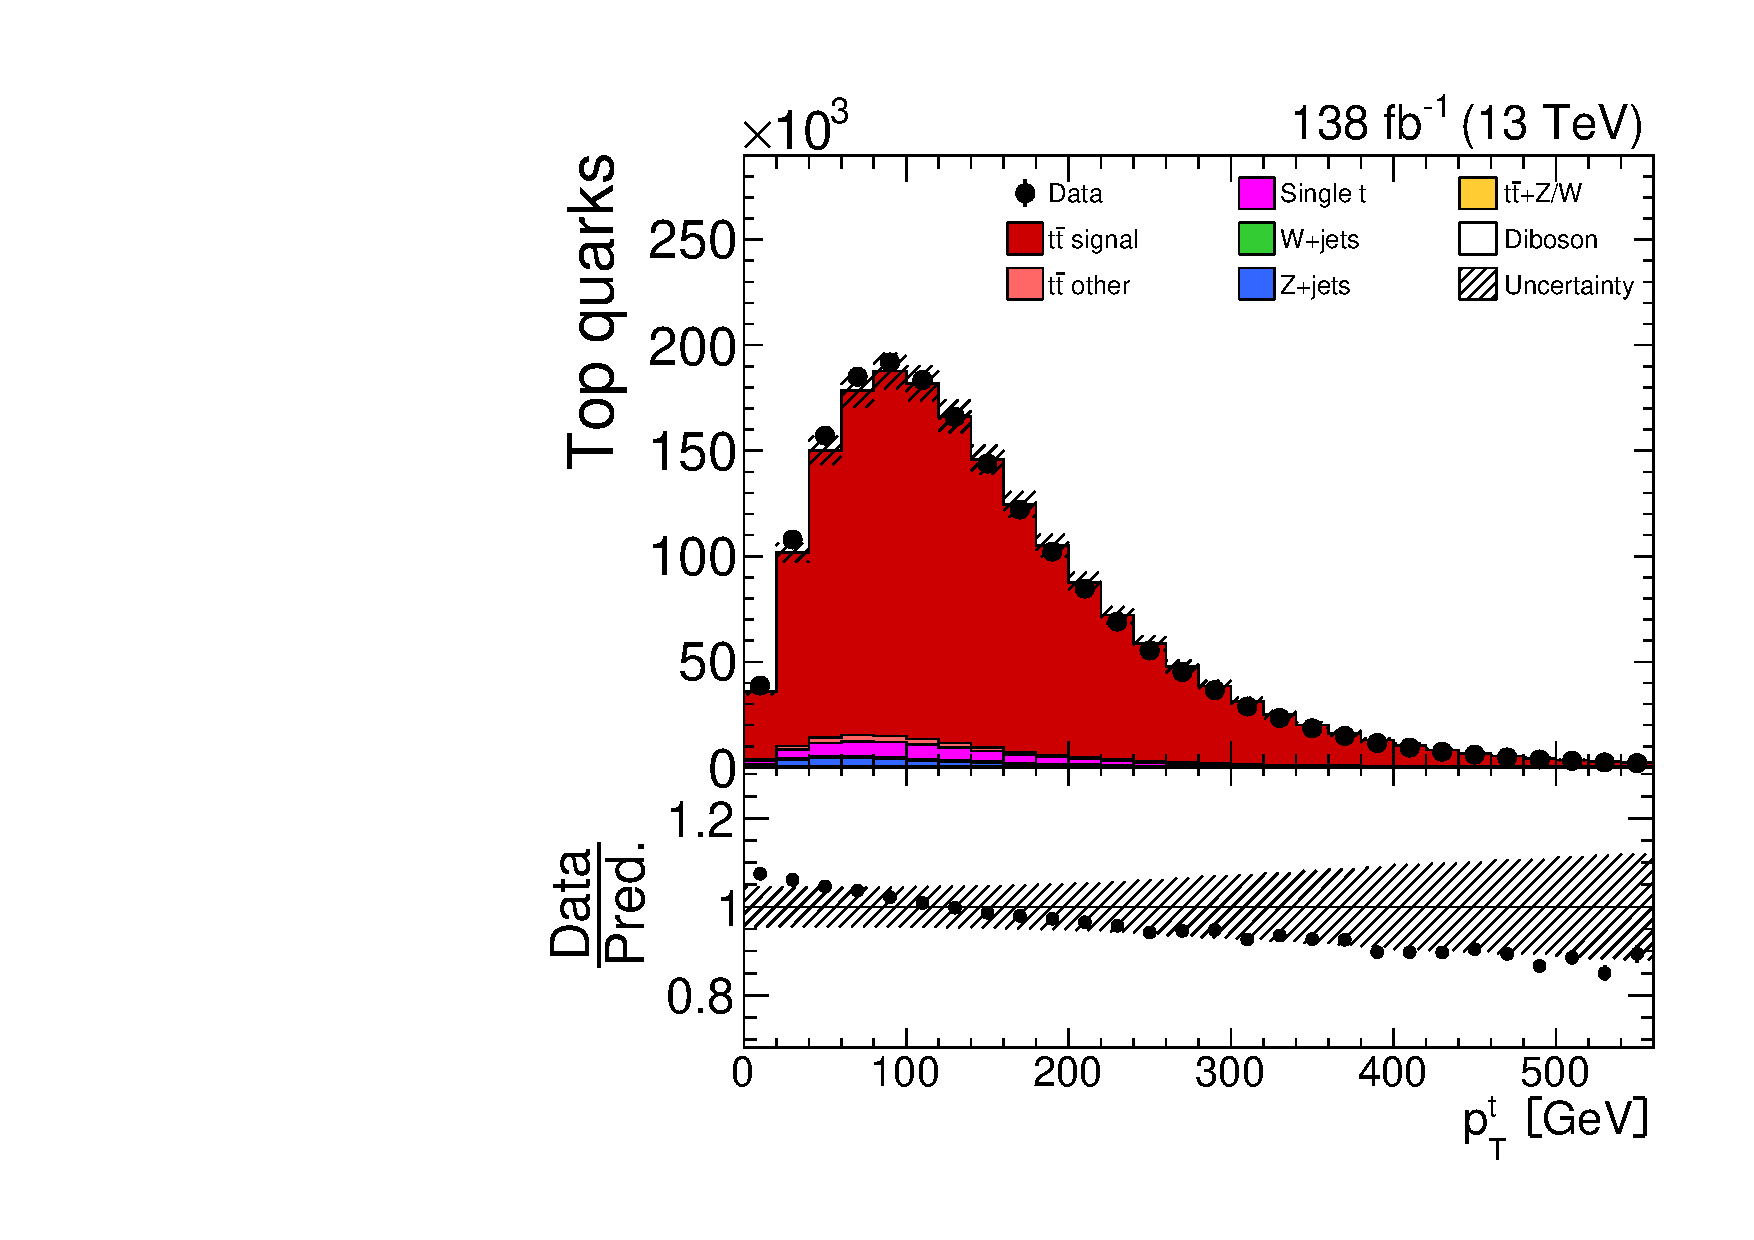
\includegraphics[width=0.30\textwidth]{fig_fullRun2UL/controlplots/combined/HypToppT.pdf}
%        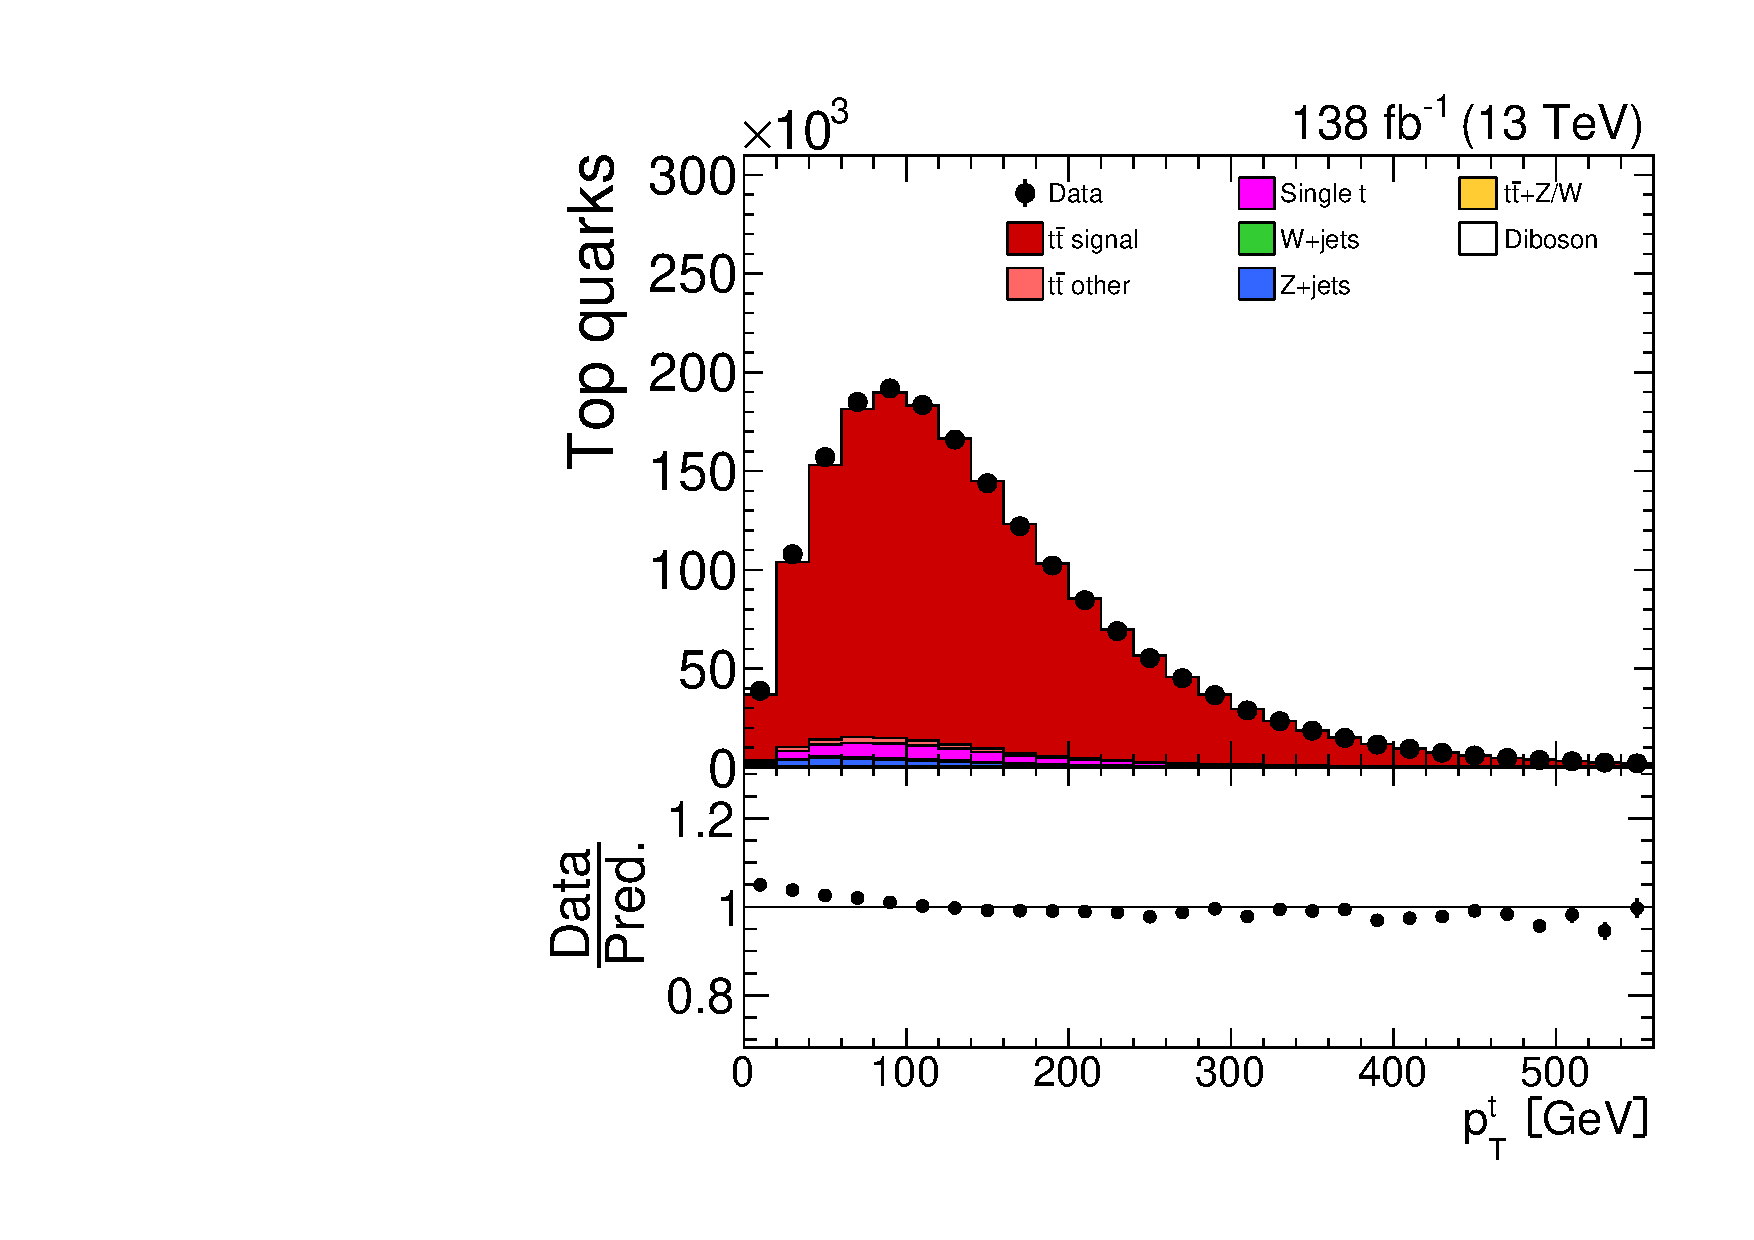
\includegraphics[width=0.30\textwidth]{fig_fullRun2UL/TOP_PT/combined/HypToppT.pdf}
      \end{center}
      \caption{\small Distribution of top \pT for Full Run II in the combined channel before (left) and after (right) top \pT reweighting.}      
      \label{fig:fullRun2ULtopptreweighting}
    \end{figure}
\end{itemize}
















